\chapter{Evaluation}

First of all, the accuracy of the model was tested agaist the testing subset provided by the used dataset. The following groups of images show the loss (left) and
the accuracy (right) at each epoch.

\begin{figure}[H]
\centering
\begin{minipage}{.45\textwidth}
  \centering
  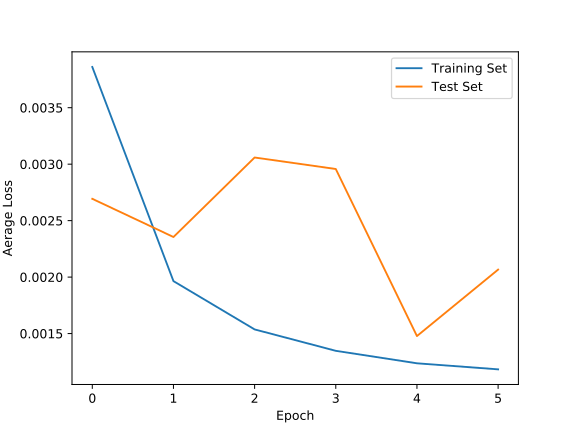
\includegraphics[width=\linewidth]{model_losses_default.png}
  \caption{Default Model Losses - Training}
\end{minipage}
\begin{minipage}{.45\textwidth}
  \centering
  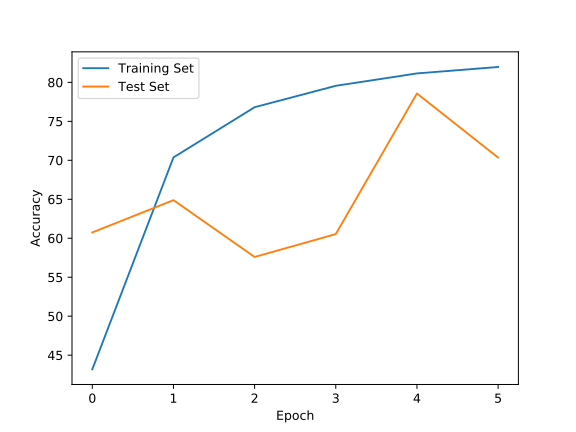
\includegraphics[width=\linewidth]{model_accuracies_default.png}
  \caption{Default Model Accuracies - Training}
\end{minipage}
\end{figure}

Interestingly, the testing accuracy seems to fluctuate and even decreases by a bit at the end while the training accuracy still keeps growing. But still, with
the testing dataset reaching a 78.1\% accuracy and the training dataset reaching a accuracy of 82.5\%, the goal is definetly reached. For reference, the same model
is tested against the validation dataset to see if there are differences in data quality.

\begin{figure}[H]
\centering
\begin{minipage}{.45\textwidth}
  \centering
  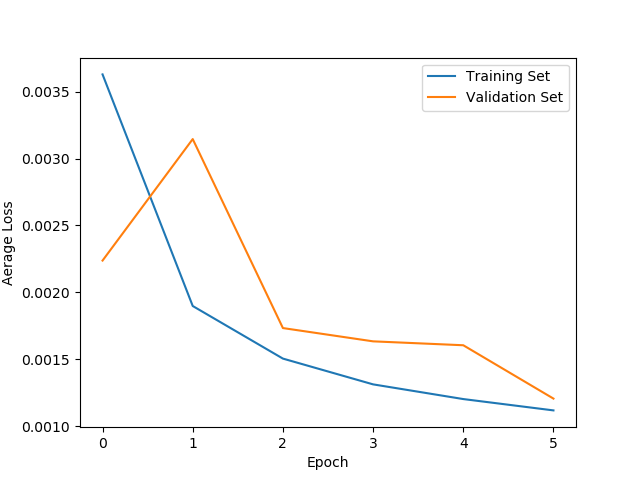
\includegraphics[width=\linewidth]{model_losses_validation.png}
  \caption{Default Model Losses - Validation}
\end{minipage}
\begin{minipage}{.45\textwidth}
  \centering
  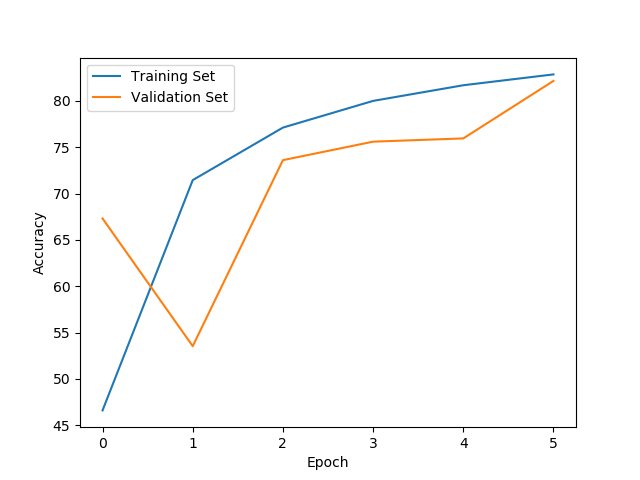
\includegraphics[width=\linewidth]{model_accuracies_validation.png}
  \caption{Default Model Accuracies - Validation}
\end{minipage}
\end{figure}

Here, a bit smoother curve for the validation dataset can be seens with the training set reaching 82.9\% and the validation set reaching 82.2\%. With the relativly small epoch
count and it being relativly close to the testing accuracy, it is concluded that no difference in data quality exists. In the next step, the the model is evaluated
with background noise. The following table shows the maximum accuracies for different noises provided by the dataset mixed into the original testing audio at different percentages.

\begin{table}[H]
  \begin{center}
    \begin{tabular}{l|l}
      Percentage & Exercise Bike & Running Tap & White Noise\\\hline
      50 & 76.9 & 68.8 & 70.1\\
      75 & 66.1 & 62.8 & 55.9\\
    \end{tabular}
    \caption{Background Noise Accuracies}
  \end{center}
\end{table}

TODO: constant noise, no sudden spikes and full canceling of original audio, no guarantee that amplitude (audio volume) is the same, so might not be equal parts mixed togther
TODO: still shows great 